\section{Welle-Teilchen-Dualismus}
\authors{Patricia Mühren, Kristina Heuser}

Das Doppelspaltexperiment mit Photonen und Elektronen sowie der photoelektrische Effekt zeigen auf, dass Licht und Elektronen sowohl Wellen- als auch Teilchencharakter haben.

Zunächst kann das Doppelspaltexperiment mit Kugeln veranschaulicht und theoretisch betrachtet werden. Dabei werden Kugeln von einer Quelle ausgesendet und passieren zwei schmale, parallele Spalten. Auf einem Beobachtungsschirm in einiger Entfernung kann man daraufhin erkennen, dass die Verteilung beziehungsweise die Ankunftswahrscheinlichkeit für klassische Teilchen der Summe der beiden Einzelspaltverteilungen entspricht (vergleiche Abbildung \ref{dsafigure:beispiel1}). Im nächsten Schritt wird das Gedanken-Doppelspaltexperiment mit Wellen ausgeführt. Hier weist die Verteilung ein Interferenzmuster auf. Dies lässt sich dadurch erklären, dass die Maxima der Verteilungsfunktion genau an den Orten konstruktiver Überlagerung liegen (vergleiche Abbildung \ref{dsafigure:beispiel2}). 

\begin{dsafigure}
\centering
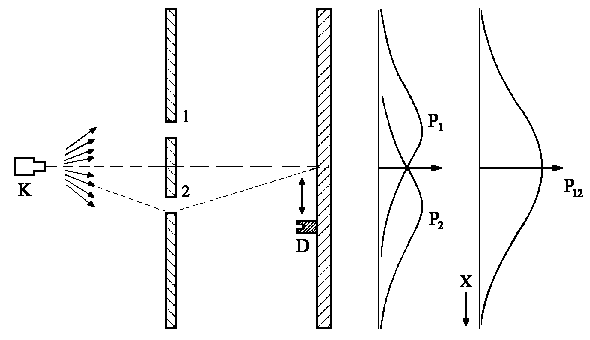
\includegraphics[scale=0.5]{Kugeln.png}
\caption{Das Doppelspaltexperiment mit Kugeln. \cite{Doppelspalt}}
\label{dsafigure:beispiel1}
\end{dsafigure}

\begin{dsafigure}
\centering
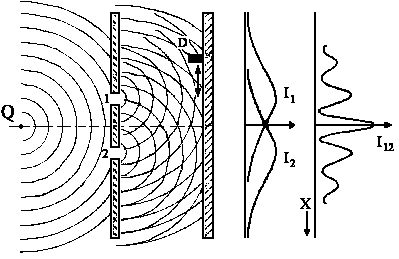
\includegraphics[scale=0.5]{Wellen.png}
\caption{Das Doppelspaltexperiment mit Wellen. \cite{Doppelspalt}}
\label{dsafigure:beispiel2}
\end{dsafigure}

Die Durchführung des Experimentes mit Elektronen zeigt, dass die Verteilungsfunktion der Elektronen nicht der Summe der beiden Einzelspaltverteilungen entspricht, wie sich Abbildung \ref{dsafigure:beispiel3} entnehmen lässt. Daher weisen Elektronen Welleneigenschaften auf. Ebenso zeigt Licht im Doppelspaltexperiment Interferenzen und, einhergehend damit, auch die Eigenschaften einer Welle. 

\begin{dsafigure}
\centering
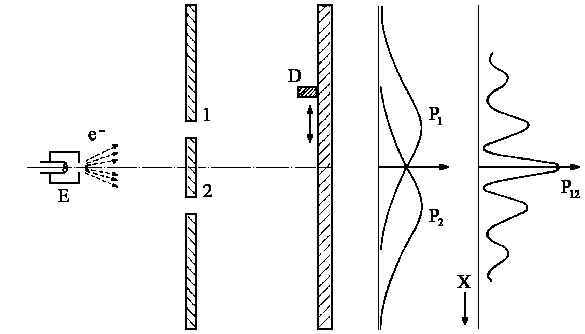
\includegraphics[scale=0.5]{Elektronen.png}
\caption{Das Doppelspaltexperiment mit Elektronen. \cite{Doppelspalt}}
\label{dsafigure:beispiel3}
\end{dsafigure}

Paradoxer Weise illustriert der photoelektrische Effekt, bei dem durch Auftreffen von Licht auf eine Metalloberfläche Elektronen emittiert werden, dass Licht ebenso Teilchencharakter aufweist, der der Wellennatur zuwider zu laufen scheint. Die Beobachtung gleichbleibender Energie der emittierten Elektronen bei zunehmender Intensität des Lichtes widerspricht der aus der klassischen Wellenbeschreibung abgeleiteten Folgerung, dass eine Zunahme der Intensität zu einem Anstieg der kinetischen Energie des herausgelösten Elektrons führen müsste. Dieser Umstand kann mit Teilchencharakter von Elektronen erklärt werden. Analog dazu wird derselbe Versuch mit Elektronen realisiert -- mit dem gleichen Ergebnis wie bei Licht.
Die Tatsache, dass Licht und Elektronen sowohl Wellen-, als auch Teilchencharakter besitzen, wird mit dem Welle-Teilchen-Dualismus addressiert. Sie ist aus einer rein klassischen Anschauung heraus nicht zu erklären und fordert eine neue Theorie \cite{Feynman_lectures70}.


